%\lhead{Modulok es kapcsolatok}

\section{Alacsony szintű modulok} 

A robot alacsonyszintű feladatait, amelyek a motor hajtásához kapcsolódó szenzorokat és vezérlő jelek előállítására hivatott a két darab CmodA7 20T FPGA fejlesztőlap. Négy tengely szögsebességét kel szabályozni, egy FPGA két hajtást valósít meg. A \ref{fig:CmodA7architektura} alapján egy hajtáshoz tartozó I/O-k:

\begin{table}[H]
\center
\begin{tabular}{lll}
\hline Név                            & Darab              & Típus  \\ \hline
Inkrementális enkoder           & 2           & Digitális Input \\
Árammérő szenzor                & 1                  & Analóg Input \\
Motor vezérlő                   & 3                  & Digitális Output \\
Végálas kapcsoló                 & 1                  & Digitális Input        
\end{tabular}
\end{table}




\renewcommand{\img}{SajatRobot/SzerkAbrak/cmoda7modulok.jpg}
\renewcommand{\sources}{*}
\renewcommand{\captionn}{CmodA7 FPGA-ban kialakított architektúra amely a szenzorok és motor hajtások kezelésre hivatott }
\renewcommand{\figlabel}{CmodA7architektura}
\begin{kep}
\begin{figure}[H]
\centering
\ifthenelse{\equal{\svg}{*}}
{
    \includegraphics[width=\aspectratioPic\textwidth,angle=\rotationAnglePic]{\img}
}
{
    \includesvg[width=\aspectratioPic\textwidth,angle=\rotationAnglePic]{\img}
}

 \ifthenelse{\equal{\sources}{*}}
    { \captionof{figure}{ \captionn}}
    { \captionof{figure}{ \mand{\mand{\captionn}{Forrás:}}{}} }
  	

\ifthenelse{\equal{\figlabel}{*}}
    {}
    {\label{fig:\figlabel}}%
    
\renewcommand{\figlabel}{*}



\end{figure}
\end{kep}
\renewcommand{\aspectratioPic}{1}
\renewcommand{\rotationAnglePic}{0}
\renewcommand{\svg}{*}



A \ref{fig:VivadoHl} a Vivado tervezőprogramban FPGA- ban megvalósított processzor architektúra látható, tartalmaz egy szoft core processzort (microBlaze) a Xilinx. Az utasítás és az adatmemória az $microblaze\_0\_local\_memory$ -ban tálalható. A memória mérete 24Kbyte 32bit sávszélességgel, amely az FPGA block memóriájából van összerakva. A programkód maga egy külső memóriában van tárolva, ami QSPI alapú interface-al kapcsolódik a FPGA hoz, az $ExternalMemorys$ kapcsolja be az AXI busz rendszeren keresztül a processzor memóriacima tartományába. A külső memória mérete 30MByte. A processzor működéséhez szükséges a $ClockAndReset$ modul előállítja az órajelet, ami 100MHz, ezen a frekvencián működik a processzor és a memória is. Az $mdm\_1$ modul a rendszerben történő jelek megfigyelésére es a processzoron futó kód debugolására hivatott.

A \ref{fig:VivadoHl} abran lathato $UartCom$ modul belső szerkezete látható az \ref{fig:UartComVivaldo} ábrán. A modula $uartcommand\_0$ szerepe a kommunikációs protokoll implmentálása hardveres szinten, a modul fogadja az UART protokollon 8bit csomagokat. A protokoll által meghatározott keretezési bytokat figyelve (Start,Stop,Skip). Ezek paraméterként megadhatok a microBlaze proceszoron keresztül. A processzor induláskor bealítja ezeket a következő értekékre: Start='S', Stop='P', es Skip='\\'. 
Start keret byte érkezésétől kezdve az öszess byte négyesével bekerül a 32bit, 400 byte-os, $blk\_mem\_gen\_0$ memóriába sorfojtonosan. Abban az esetben, ha az üzenet meghaladja a 200 byte-t, akkor a modul úgy tekinti, hogy hibás adatok érkeztek és visszatér a kiinduló állapotba. Abban az esetben, ha bináris adatokat küldünk, tartalmazhat speciális protokoll keretezésben resztvevő karaktereket,  így ezeket eloti karakter Skip kell hogy legyen. A skip karakterek nem kerülnek bele a memóriába ezeket a hardver kiveszi.


A kommunikació  folyamatát a \ref{fig:FPGAuartRos} ábrán is végig követhetjük.

\begin{figure}[H]		
		%trim = bal also jobb felso
   \fbox{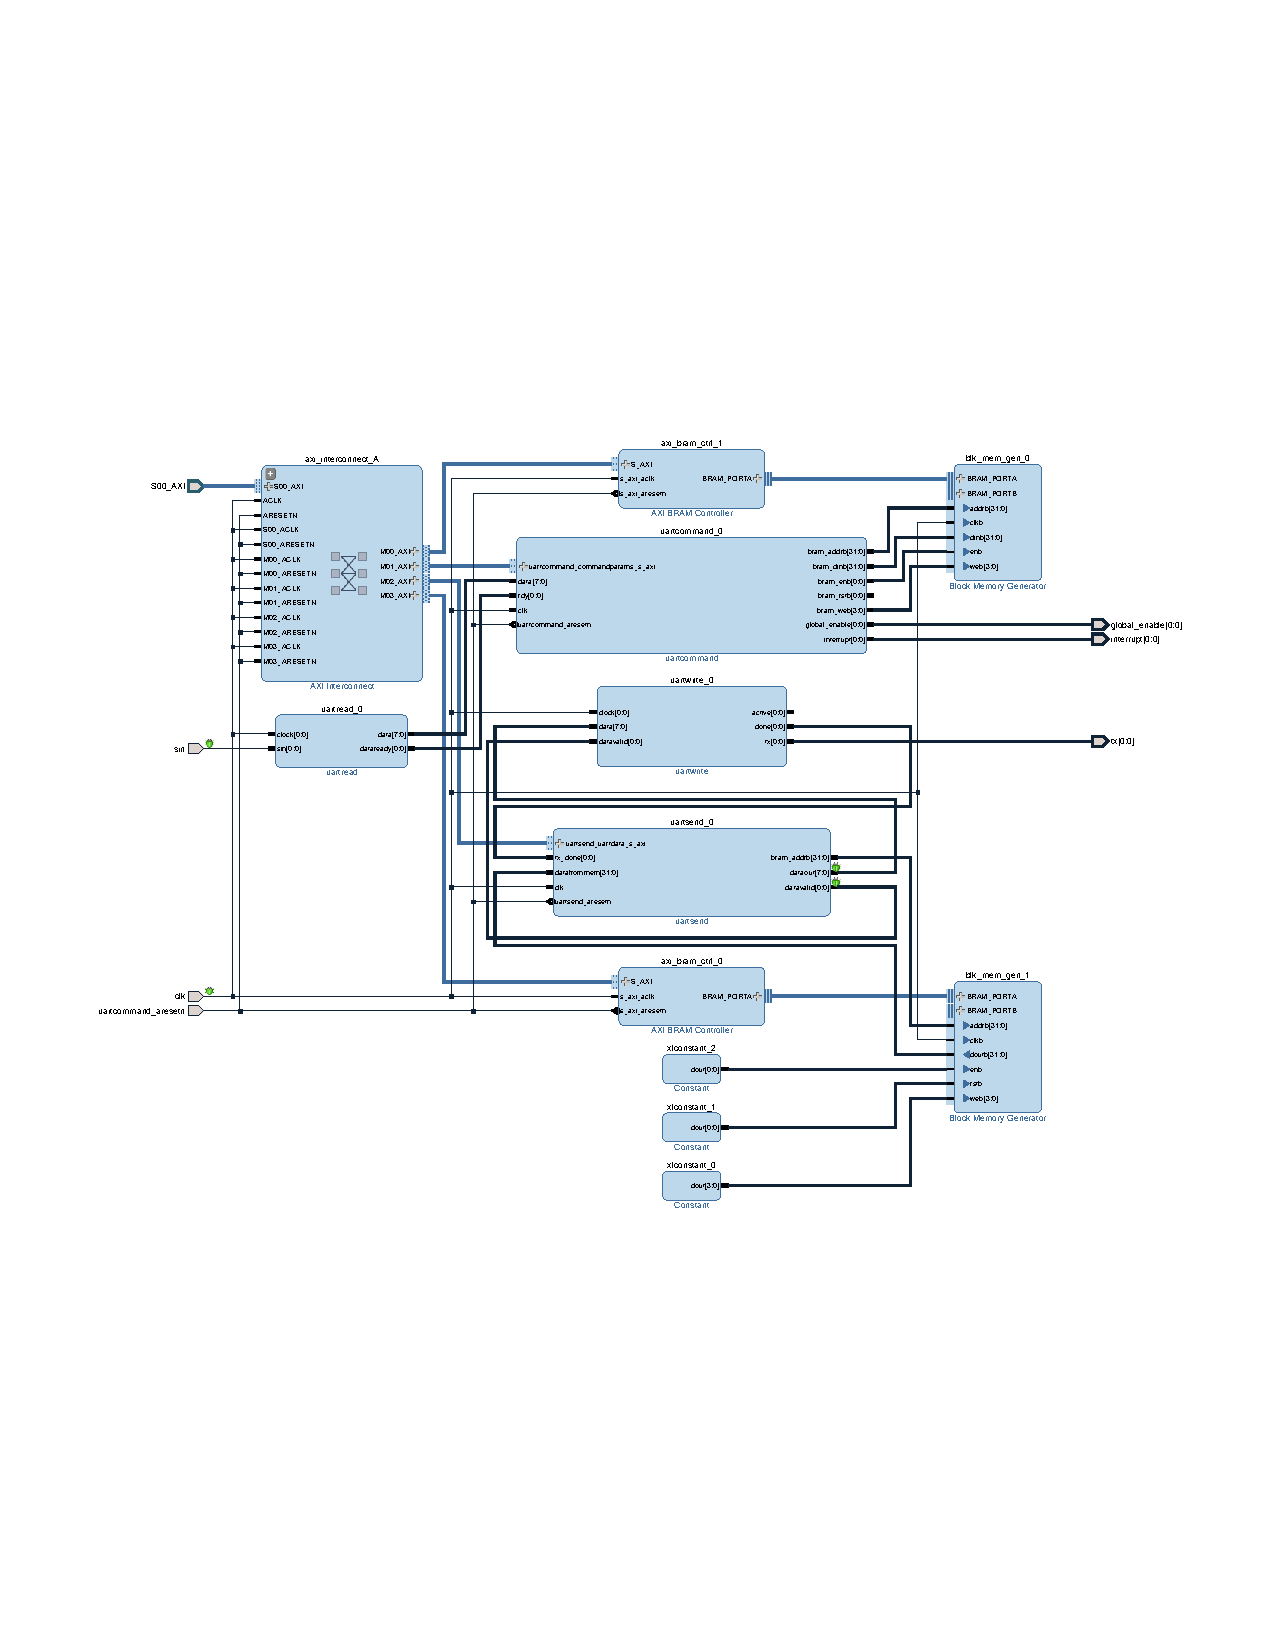
\includegraphics[width=1.1\columnwidth,trim=3cm 7cm 1cm 7cm,clip]{tikz/UartCom.pdf}}
  \caption{FPGA ban megvalositott komunikacios protokol a 	     \ref{fig:FPGAcomuSection} leirt protokol alapjan.}
  \label{fig:UartComVivaldo}
\end{figure}


\renewcommand{\img}{SajatRobot/FPGAmodulok/UartUML.jpg}
\renewcommand{\sources}{*}
\renewcommand{\captionn}{FPGA hardver/MicroBlaze processzor és ROS node közötti kommunikáció megvalósitása UART protokoll alapján }
\renewcommand{\figlabel}{FPGAuartRos}
\begin{kep}
\begin{figure}[H]
\centering
\ifthenelse{\equal{\svg}{*}}
{
    \includegraphics[width=\aspectratioPic\textwidth,angle=\rotationAnglePic]{\img}
}
{
    \includesvg[width=\aspectratioPic\textwidth,angle=\rotationAnglePic]{\img}
}

 \ifthenelse{\equal{\sources}{*}}
    { \captionof{figure}{ \captionn}}
    { \captionof{figure}{ \mand{\mand{\captionn}{Forrás:}}{}} }
  	

\ifthenelse{\equal{\figlabel}{*}}
    {}
    {\label{fig:\figlabel}}%
    
\renewcommand{\figlabel}{*}



\end{figure}
\end{kep}
\renewcommand{\aspectratioPic}{1}
\renewcommand{\rotationAnglePic}{0}
\renewcommand{\svg}{*}


\begin{figure}[H]
  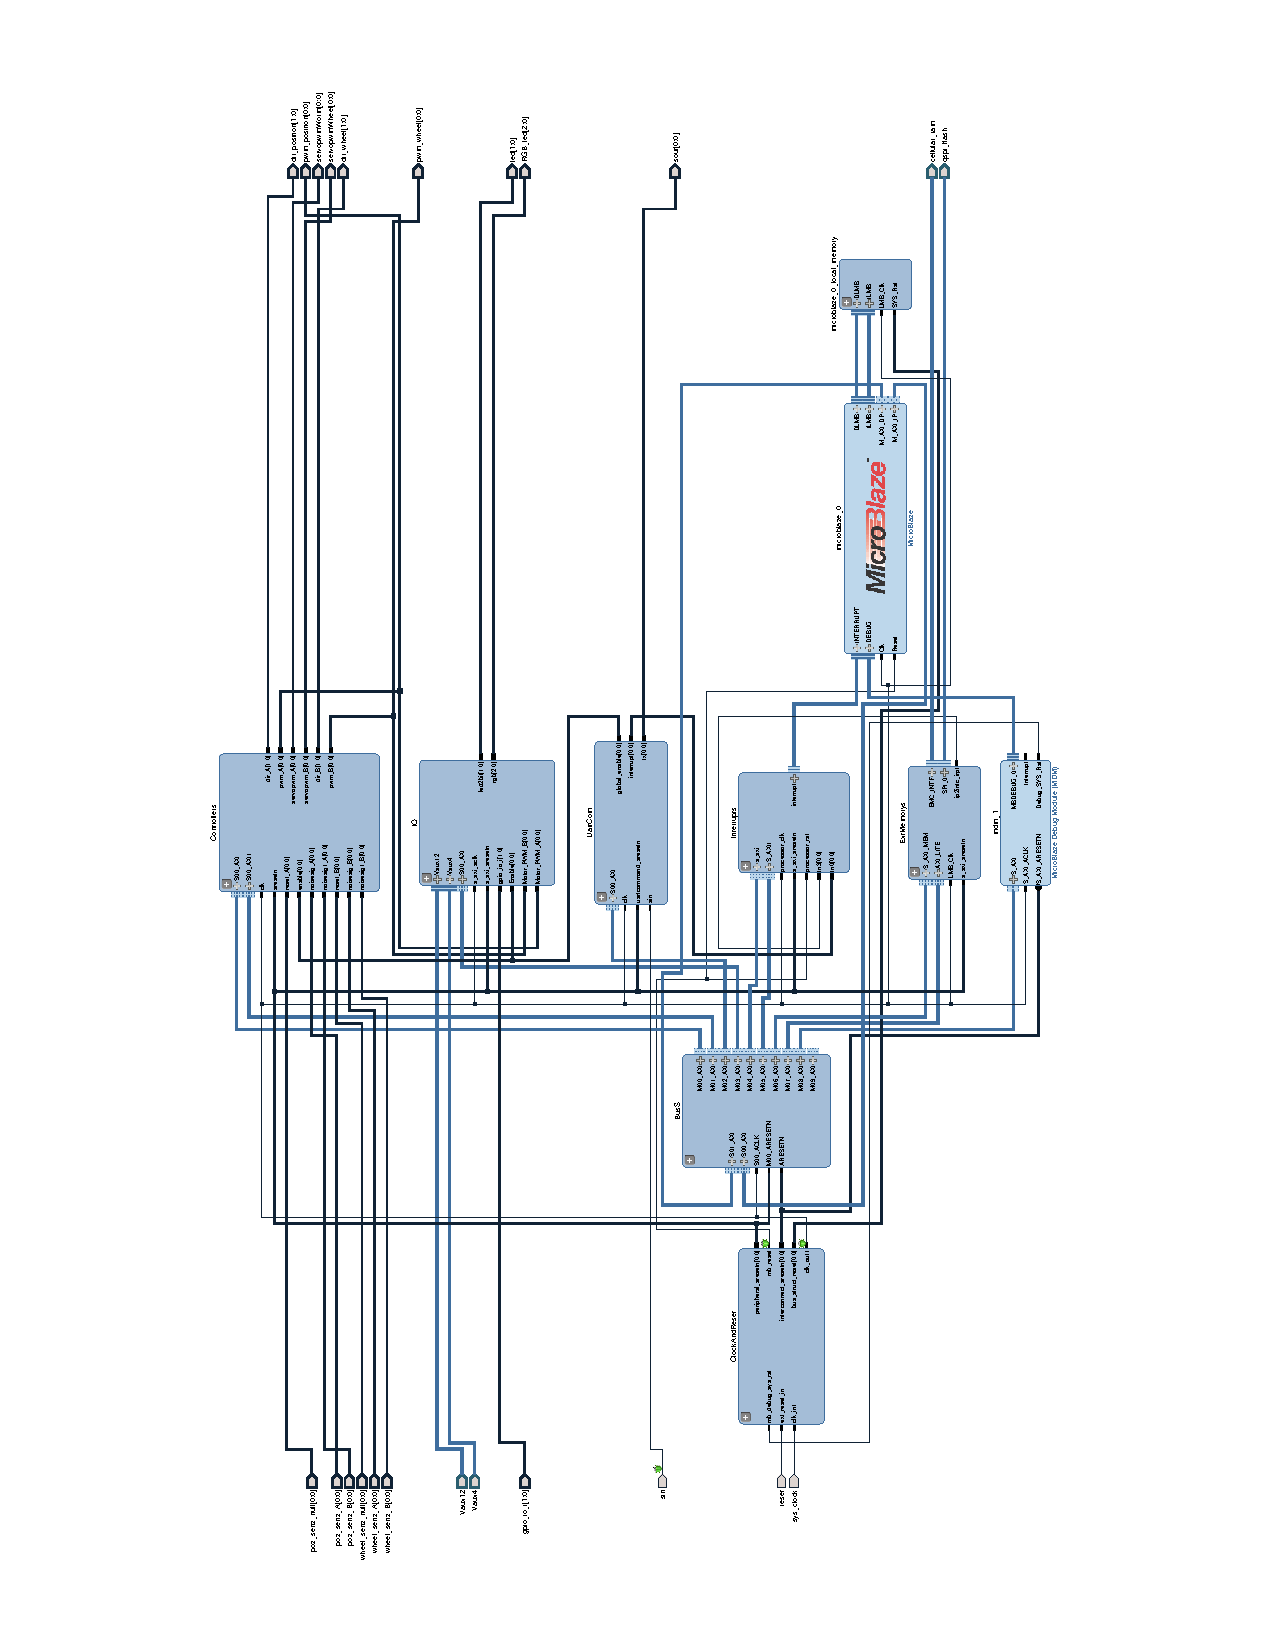
\includegraphics[width=1.2\columnwidth]{tikz/VivadoHL.pdf}
  \caption{FPGA ban megvalósitott szoftproceszor rendszer, legfelső négyzet.}
  \label{fig:VivadoHl}
\end{figure}

A keret veget jelzo byte erkezesekor a modul general egy megszakitast a microBlaze proceszornak az $interupt[0:0]$ kivezetesen keresztul.
A megszakitas kiszolgalasakor a proceszor kiolvasa az $uartcommand_0$ modulbol az uj uzenet kezdocimet. A proceszor az adatokat az $axi\_bram\_ctrl\_1$ modulon keresztul kepes kiolvasni, az uj uzenetre mutato pointer erteket megkapjuk, ha az $uartcommand_0$ modul proceszor memoriajaba illesztett kezdocimet es a modul altal jelzet kezdocimet osszeadjuk.
Abban az esetben, ha az adatok feldolgozasa elott uj csomag erkezik a hardver komunikacios modulhoz, elkezdodik annak beirasa a memoriaba, az elozo adatok felulnemirasaval.

A $uartcommand_0$ modul kimenete $global\_enable[0:0]$ engedelyezo jel, abban az esetben ha nemkap a hardver $SREP$ uzenetet legalabb 300ms kent akkor az engedelyezo jelet alacsonyra alitja vagy ha $SRDP$ uzenet erkezett.

Az $uartsend\_0$ modul hasonlokeppen mukodik csak az adatok kuldesere hivatott. A microBlaze proceszor az $axi\_bram\_ctrl\_0$ modulon keresztul beleirodnak a $blk\_mem\_gen\_1$ \cite{DualPortRam} 32bites es 400byte meretu meoriaba.
Az iras vegevel a proceszor bealitja a kuldes felget, amely egy parameter a hardvernek. A modul elkezdi kikuldeni az adatokat. Abban az esetben ha a csomag tartalamz szpecialis protokolt leiro byte-t akkor a modul automatikusan elkuldi elote a Skip karaktert.

Az $uartread\_0$ az UART protokol implemetalja FPGA hardverebe, a $sin$ az RX bemenet, a $data[7:0]$ a 8bite szeles adatvezetek ami tartalmaza az utolso berkezet byte uzenetet. A $dataready[0:0]$ felfuto el jelzi az uj adat erkezeset. Az $uartwrite\_0$ modul a $data[7:0]$ 8bites sinen erkezo adatot kuldi ki UART protokol alapjan a $tx[0:0]$ kimenetere abban az esetben ha a $datavalid[0:0]$ bemeneten egy felfuto el erkezik.

Az \ref{fig:ControllersVivado} hathato $A$ es $B$ modul feladatuk egy-egy DC motor szabalyzasat lassak el. Mindket modulban ugyan azon alegysegek talalhatok meg az $A$ modul az robot elso, mig a $B$ modul a robot hatso kereket szabalyozza.

A \ref{fig:ControllerMag} abran lathato a modulok belso szerkezete. A $pwm\_hardver\_B$ PWM jelet allit a $pwm[0:0]$ kimeneten, es egy iranyjelet $dir[0:0]$ a bemeneti 16bites elojeles szambol. A PWM kitoltesi tenyezoje -32000 tol 32000 ig terjed ki az elojel meghatarozza az iranyt mig az abszolut erteke a pwm kitoltesi erteket. A $enable[0:0]$ jel engedelyezi a kimenetet, ha erteke alacsony akkor a pwm kimenet is alacsony.


\begin{figure}[H]
  		%trim = bal also jobb felso
   \fbox{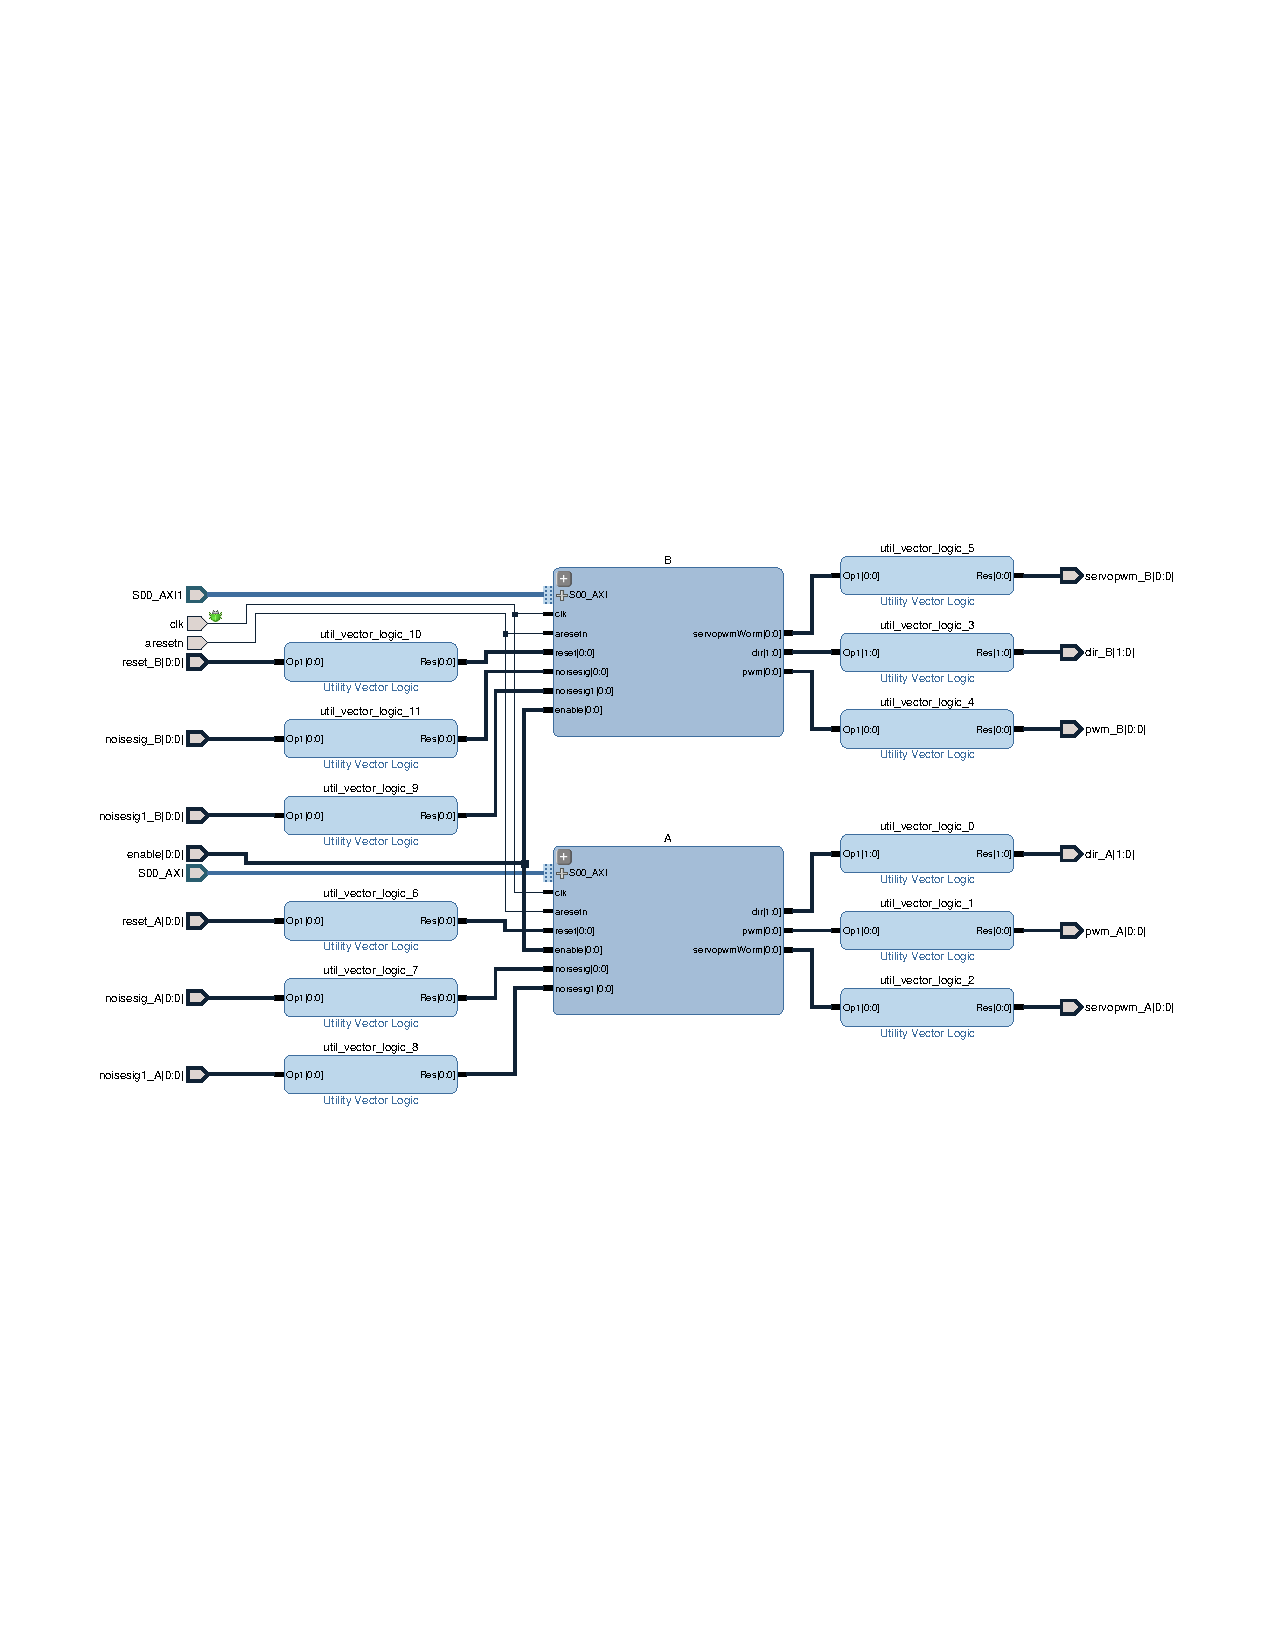
\includegraphics[width=1.1\columnwidth,trim=2cm 9cm 1cm 9cm,clip]{tikz/Controllers.pdf}}
  \caption{FPGA ban megvalositott szabalyzok A es B}
  \label{fig:ControllersVivado}
\end{figure}

Az $InkrementalisSensor\_B$ axi sinen keresztul kapcsolodik a proceszorhoz, feladata az inkrementalis szenzortol erkezo $A$ es $B$ jeleknek a feldolgozasa. A modul ket jelet kuld ki: $dir[0:0]$ amely a forgas iranyat jelzi, $imp[0:0]$ egy orajelperiodusig tarto felfutojelet kuld ki az inkrementalis szenzor minden egyes elmozdualsara.
\begin{figure}[H]
    		%trim = bal also jobb felso
   \fbox{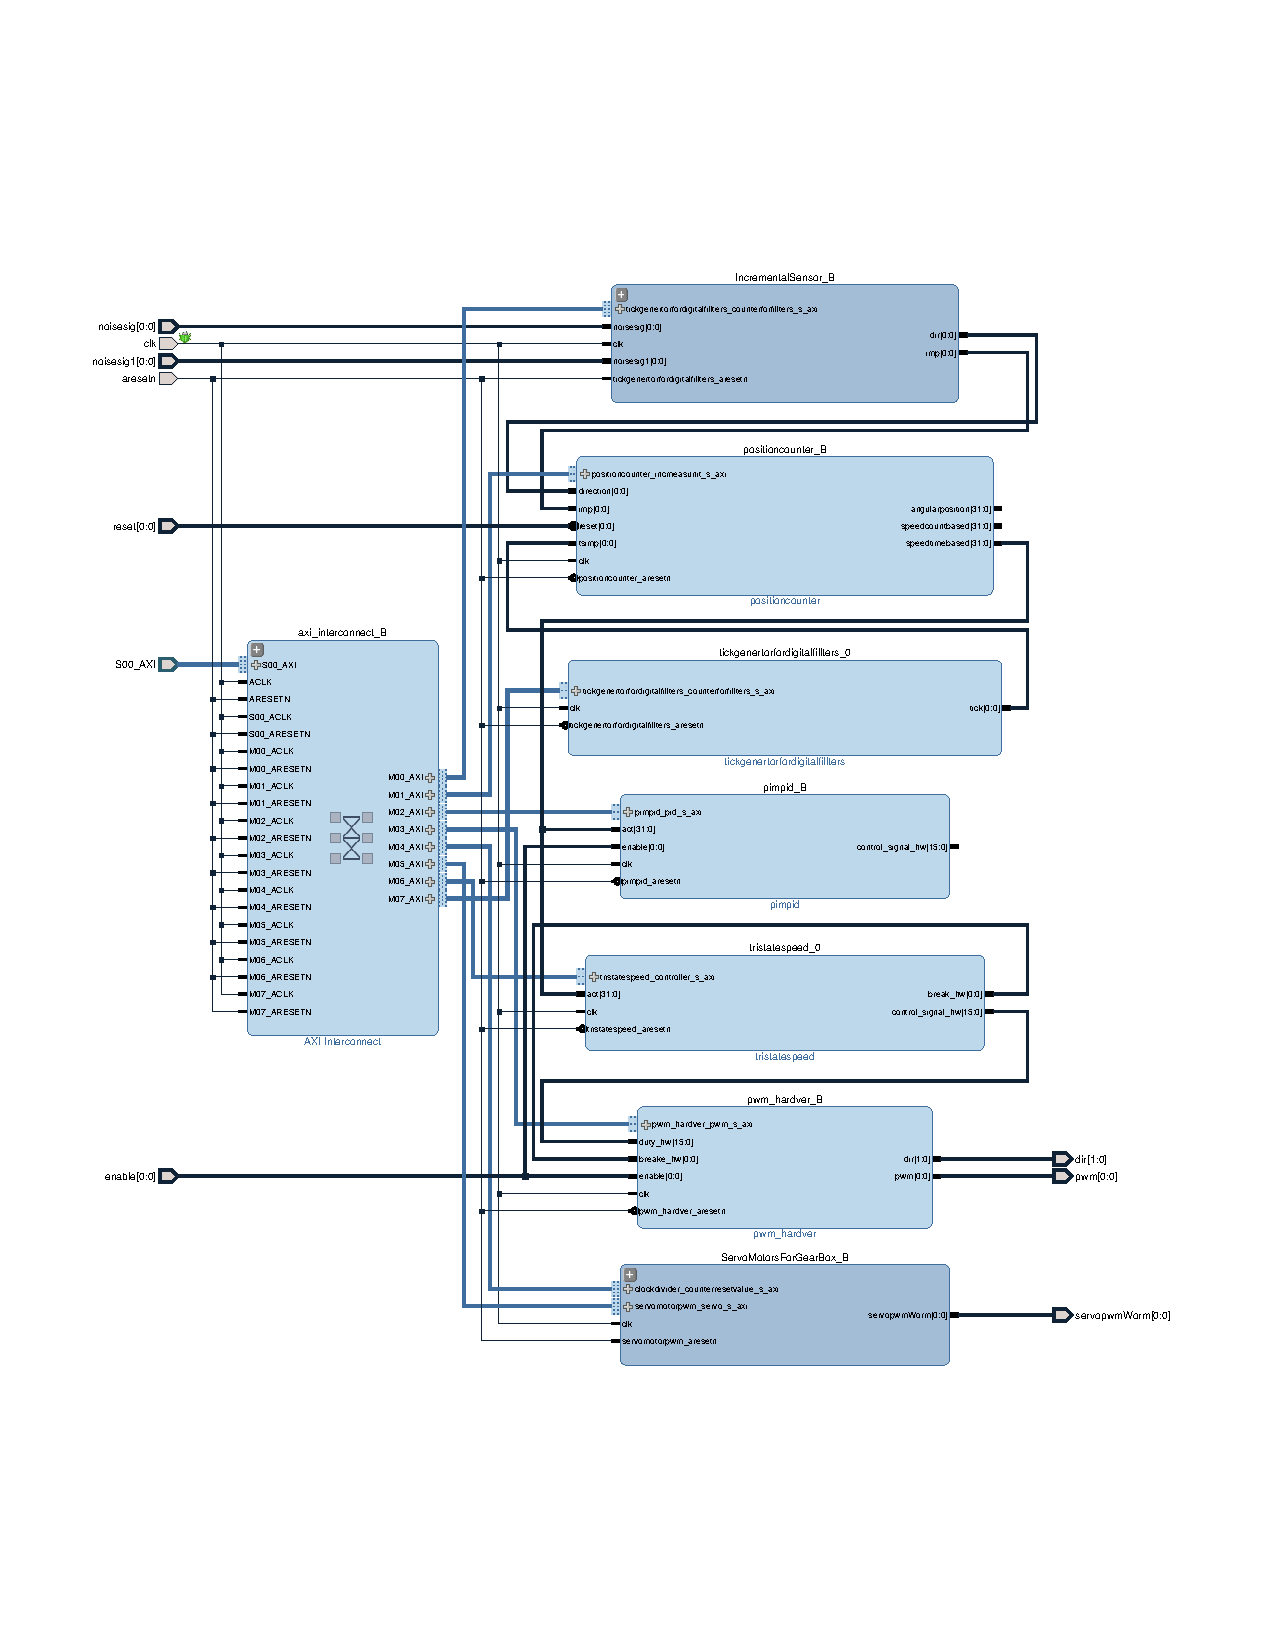
\includegraphics[width=1.1\columnwidth,trim=1cm 4cm 1.8cm 4cm,clip]{tikz/B.pdf}}
  \caption{FPGA controller mag.}
  \label{fig:ControllerMag}
\end{figure}

A $positioncounter\_B$ modul meri a szogsebeseget es a szogpoziciot ido es impulzus szamolasi modszereket hasznalva. A proceszor a sajat mintaavetelezesi frekvenciajaval olvassa ki a modulbol a mert ertekket es alakitja at a kivant mertekegyszegekbe.

Az \ref{fig:ControllerMag} abran lathato tobbi modul jelen pilanatban tovabfejlesztesi lehetosegkent jeleni meg. A $pimpid\_B$ modul FPGA alapu PID szabalyzo modul, $ServoMotorGearBox\_B$ a DC motrokon levo fogaskerek kapcsolasi lehetoseget hivatott majd alitan egy szervomotor segitsegevel.

A szabalyzok referencia ertekeit a $RefValues$ funkcionalitas biztositja, a megfelelo uzenetek erkezesekor a memoriaba bealitodnak a kivant referencia ertekek, es majd a szoftveres szabalyzok innet olvasak ki. A hardveres szabalyzoknak pedig a beerkezes pillanatban lekuldodik a hardveres moduloknak.

A $Monitors/Controllers$ funkcionalitas egy parameterbol allithato periodusu idozito amely megszakitasokat general a proceszornak. A proceszor ezekre a megszakitasokra szamolja ki a beavatkozi jelek uj ertekeit, valamint a elkuldi a mert,es a kapott referencia erteketk UART on keresztul.



\subsection{Microblaze szoftvere}

A rendszer tervezesenel a fo koncepcio az volt hogy a rendszer arhitekturaja dinamikus legyen a fejleszhetoseget tekitve, igy a \ref{fig:CmodA7architektura} levo arhitekurat kaptuk.

A microblaze proceszor feladatai hardveres modulok kezdeti allapotainak a beallitasa, szoftveresen furt szabalyzot mukodtetese, az beerkezett uzenetek feldolgozasa. A proceszoron futo szoftvert az \ref{fig:MicroblazeSoft} UML diagram szemleteti.
A peremeterek irasa es olvasasa funkcionalitasban, az ujonan erkezet parameter ertkenek a bealitasi mente a kovetkezo: az uzenet beleirodik a memoriaba, megszakitas generalodik a proceszor iranyaban, a procesyor feldolgozza az uj uzenetet, eszleli hogy parameter ertekenek a bealitasa tipusu uzenet erkezett, meghivodik az eszt kiszolgalo fuggveny. A tovabiakkban az osszes parameter ujraszamolodik, es ujrakuldodik a hardveres modulok iranyaba. Abban az esetben ha minden sikeresen zajlot a proceszor pozitiv viszajelzst(ACK) uzenetet kuld es viszakulde a bealitott parameter erteket, acelbol hogy a kuldo is megbizonyosodhadjon a parameter helyes bealitasarol.


\renewcommand{\img}{SajatRobot/FPGAmodulok/uBlazeAndFpgaUML.jpg}
\renewcommand{\sources}{*}
\renewcommand{\captionn}{MicroBlaze proceszoron futo szoftver diagramja}
\renewcommand{\figlabel}{MicroblazeSoft}
\begin{kep}
\begin{figure}[H]
\centering
\ifthenelse{\equal{\svg}{*}}
{
    \includegraphics[width=\aspectratioPic\textwidth,angle=\rotationAnglePic]{\img}
}
{
    \includesvg[width=\aspectratioPic\textwidth,angle=\rotationAnglePic]{\img}
}

 \ifthenelse{\equal{\sources}{*}}
    { \captionof{figure}{ \captionn}}
    { \captionof{figure}{ \mand{\mand{\captionn}{Forrás:}}{}} }
  	

\ifthenelse{\equal{\figlabel}{*}}
    {}
    {\label{fig:\figlabel}}%
    
\renewcommand{\figlabel}{*}



\end{figure}
\end{kep}
\renewcommand{\aspectratioPic}{1}
\renewcommand{\rotationAnglePic}{0}
\renewcommand{\svg}{*}





\subsection{FPGA es UART alapu komunikacios protokol}
\label{fig:FPGAcomuSection}
Megvalositva a komunikaciot a kiszolgalo ROS noddal, amely UART protokolra epitett sajat uzenetekbol all \ref{fig:FPGAComCsomagAlt}.

\renewcommand{\img}{SajatRobot/FPGAmodulok/ProtokolDiagram.jpg}
\renewcommand{\sources}{*}
\renewcommand{\captionn}{FPGA komunikacios protokol altalanos csomag szerkezet}
\renewcommand{\figlabel}{FPGAComCsomagAlt}
\begin{kep}
\begin{figure}[H]
\centering
\ifthenelse{\equal{\svg}{*}}
{
    \includegraphics[width=\aspectratioPic\textwidth,angle=\rotationAnglePic]{\img}
}
{
    \includesvg[width=\aspectratioPic\textwidth,angle=\rotationAnglePic]{\img}
}

 \ifthenelse{\equal{\sources}{*}}
    { \captionof{figure}{ \captionn}}
    { \captionof{figure}{ \mand{\mand{\captionn}{Forrás:}}{}} }
  	

\ifthenelse{\equal{\figlabel}{*}}
    {}
    {\label{fig:\figlabel}}%
    
\renewcommand{\figlabel}{*}



\end{figure}
\end{kep}
\renewcommand{\aspectratioPic}{1}
\renewcommand{\rotationAnglePic}{0}
\renewcommand{\svg}{*}



A protokol keretek koze foglalt adatok sorendisegere epul. Szpecialis karakterek \footnote{specialis karakterek amelyek jelzik az ertelmezo szamara hogy olyan karakter kovetkezik amelyet a protokol ertelmezeseben nem kell vegrehajtani.} jelzik az uzenet kezdetet es veget jelen esetben az $S$ csomag kezdetet, mig a $P$ a csomag veget jelentik.
Az csomag tartalmazhat binaris formatumo adatot is ezeket minden esetben a \{ es \} szpecialis karakterek koze kel kerulniuk, mert a koztuk levo adat nem fog ertelemzesre kerulni a feldolgozo altal. Binaris reszt  pl:. struktura tipusu adatra hasznalhatjuk. Mindig a \{ utani elso karakter megadja a binaris adat hoszat igy tudja az ertelmezo hogy hol kell varnia a lezaro karaktert. A binaris szekco hossza nemlehet nagyobb mint 254 byte hosszu, de amenyiben szukseges kiterjeszheto.

Minden uzenet tartalmaz egy egyedi azonostot ami meghatarozza az uzenet tipusat ez alapjan tudja eldonteni majd a fogad fel hogy melyik kiszolgalo rutint kell felhivnia. Ezt koveti egy uzenet szamlalo 5 char hoszu mezo amely string formaban tartalmez egy egesz szamot, amley minden kikuldott uzenet utan novelni kell. Az uzenetszamlalo alol kivetelt kepeznek a direkt hardveres uzenetek pl.: $SREP$ es a $SRDP$.
A hasznos adat tovabbi felepiteset midontjuk el annak fugvenyeben hogy mit szeretnek. Jelen esetben a uzenetipus orientalt parancsokat szerkesztunk amelyekkel a referencia ertekeket, parametereket allitjuk be, valamint binaris szekciot is tartalmazo strukturat kul az FPGA a PC nek amely a szabalzast es monitorizalast szolgalja.

\subsection{Paramterek FPGA modul}

A parameterek segitsegevet tudjuk bealitani a mintavetelezesi periodusokat, az inkrementalis szenzorok felbontasat, a szabalyozok bealitasait is ezaltal oldhatjuk meg. Configuracios parameterek.: valaszhatunk szabalyzotipusokat.
Az alabbi tablazatban egy leirjuk a ROS-banhasznalt parametereket. A paremeterek nevenek vegen levo $X$ jelolje $A$ vagy $B$, attol fuggoen hogy melyik DC motorhajtashoz tartozik. Az \ref{fig:ControllersVivado}abran lathato modulokat tudjuk configuralni.
% Please add the following required packages to your document preamble:
% \usepackage{multirow}
% \usepackage[normalem]{ulem}
% \useunder{\uline}{\ul}{}

\begin{table}[H]
\begin{tabular}{lllllp{6cm}}
\hline \multirow{2}{*}{Id} & \multirow{2}{*}{\begin{tabular}[c]{@{}l@{}}Nev \\ (X lehet A vagy B)\end{tabular}} & \multicolumn{2}{l}{Ertekek} & \multirow{2}{*}{Tipus} & \multirow{2}{*}{Leiras}                                                                                                                      \\
                    &                                                                                    & Min         & Max           &                        &                                                                                                                                              \\ \hline
1                   & TsTimerPeriod                                                                      & 1           & 1000          & int16                  &  Mintavetelezesi periodus {[}ms{]} ban.                                                                                                      \\
2                   & GetDataPeriodical                                                                  & 0           & 1             & int16                  &  Kapcsolo ha 0 akkor nem kuld az FPGA mert ertekeket, kulomben a TsTimerPeriod periodusi mintavetellel kuld.                                  \\
3                   & TorqueCoefX                                                                        &             &               & float16                &  Motor aram es nyomatek kozti egyuthato.                                                                                                      \\
4                   & ActiveControllerX                                                                  & 0           & 65535         & int16                  &  Valaszhato szabalyzo tipusok hajtasonkent 0=Szoftvare PID szogsebesseg, 1=Hardver PID szogsebesseg, 2=Szoftver PID aram, 3=Hardver PID aram  \\
5                   & MaxControlSiggnalX                                                                 & 0           & 32760         & sint16                 &  A beavatkozo PWM jel maximalis kitoltesi tenyezoje, linearisan 0-\textgreater{}0\% -tol 32760-\textgreater{}100\% -ig.                       \\
6                   & IncSenzResX                                                                        & 0           & 65535         & int16                  &  Inkrementalis szenzor altal generalt inpulzusok szama egy teljes kerekfordulatra.FPGA oldalon ez a szam 10-el szorzodik.                     \\
7                   & IncSenzCountDirectionX                                                             & -1          & 1             & sint16                 &  inkrementalis szenzor jeleit feldogozo mudul szamolasi iranyanak valtoztatasara szolgalo egyuthato.                                          \\
8                   & Kp\_Whell\_PidX                                                                    & 0           &               & float16                &  szogsebeseg szabalyzo, PID erositesi parametere.                                                                                             \\
9                   & Ti\_Whell\_PidX                                                                    &             &               & float16                &  szogsebeseg szabalyzo, PID integralasi ido.                                                                                                  \\
10                  & Td\_Whell\_PidX                                                                    &             &               & float16                &  szogsebeseg szabalyzo, PID derivalasi ido.                                                                                                   
\end{tabular}
\end{table}






\subsection{Kommunikáció sebessége}

Az uart sebesege 1MBd \footnote{megabaud} ami megfelel 131072 byte/s adatforgalomnak. A valosagban a komunikacio hibatlanul mukodik 1ms periodussal kuldott 100byte hoszu uzeneteket. Osszehasonlitva $AXI\_UART\_Lite$ \cite{AXIuartLite} modullal elert eredmenyekkel 50ms periodust tudtunk csak elerni ammi annak tudhato be hogy a protoko ertelmezeset a szoftver vegezte es nem a hardver. A FIFO hasznalata elenere sem skerult nagyobb mintavetelezesi sebeseget elerni, hogy nem minden karakter utan generalt proceszor megszakitast csak minden 16-dik karakter utan.

\begin{equation}
    frekvencia = \frac{131072}{SizeOfPachage}=\frac{131072[byte/s]}{100[byte]}=1310,072 [Hz]
\end{equation}

\subsection{Biztonsagi megoldasok}

Abbana az esetben ha kikultuk az elirt ertekeket a modulnak es ezutan a komunikacio megszakadt a modullal akkor a szabalyzok probaljak tartani az elirt erteket annak elenere is hogy az mar lehet hogy ez mar nem akktualis. Erre a celra bepitesre kerult egy uzenet es egy logika (HeartBeat) amely csak a komunikacios modulhoz erkezik meg, es jelzi hogy a ROS jolmukodik, es forditva is.Abban az esetben ha a komunikacio megszakad lealitja a motrokat es a szabalyzokat,  \ref{fig:FPGAuartRos} alapjan az Enable(EN) jel.

\begin{table}[H]
\center
\begin{tabular}{lll}
\hline Irany   & Uzenet & Periodis    \\ \hline
FPGA->ROS &  SEP        & 300 ms kotelezo         \\
ROS->FPGA &  mintavetelezett ertekek kuldese & dinamikusan modosithato                   
\end{tabular}
\end{table}















